%%
%% Science Bulletin Submission — Manuscript
%% "When Benchmarks Lie: Temporal Data Leakage Reverses Anomaly Detection Rankings"
%%
%% Document class: elsarticle (Elsevier, used by Science Bulletin)
%% Bibliography style: numbered (elsarticle-num)
%%

\documentclass[preprint,12pt]{elsarticle}

%% ── Packages ──
\usepackage{amsmath,amssymb}
\usepackage{graphicx}
\usepackage{booktabs}
\usepackage{hyperref}
\usepackage{color}
\usepackage{multirow}
\usepackage{xspace}

%% ── Journal info ──
\journal{Science Bulletin}

%% ── Begin document ──
\begin{document}

\begin{frontmatter}

%% ── Title ──
\title{When Benchmarks Lie: Temporal Data Leakage Reverses Time Series Anomaly Detection Rankings}

%% ── Authors ──
\author[hnu]{Xicheng Zeng\corref{cor1}}

%% ── Affiliations ──
\affiliation[hnu]{organization={College of Finance and Statistics, Hunan University},
            addressline={Lushan South Road, Yuelu District},
            city={Changsha},
            postcode={410082},
            state={Hunan},
            country={China}}

%% ── Corresponding author ──
\cortext[cor1]{Corresponding author: Xicheng Zeng}
\ead{ZXCHGQY@hnu.edu.cn}

%% ── Abstract (≤250 words per Science Bulletin guidelines) ──
\begin{abstract}
The standard protocol for evaluating time series anomaly detection (TSAD) randomly partitions overlapping sliding windows into training and test sets. We show that this practice introduces systematic temporal data leakage that can reverse method rankings. Across five benchmark datasets (SWaT, TEP, MSL, SMAP, SMD), five methods, and three random seeds, the absolute leakage gap $|\Delta\text{AUC}| = |\text{AUC}_\text{random} - \text{AUC}_\text{temporal}|$ averages 0.080 across 25 method--dataset pairs. The distortion is both bidirectional and method-dependent: LSTM-AE loses $-$0.251 AUC on SWaT under random split, while Transformer-AE gains $+$0.150 on SMD. Ranking reversals are the critical consequence. Spearman correlations between random-split and temporal-split rankings range from $\rho = -0.7$ on SWaT (a near-perfect inversion) to $+0.8$ on SMAP and SMD; the best-performing method differs between the two protocols in four of five datasets. With nine methods, SMD reaches statistical significance ($\rho = +0.717, p = 0.030$), confirming that random-split rankings carry minimal information about honest performance even when statistical power is adequate. Under honest evaluation that partitions the raw time series before generating windows, no single method dominates across all benchmarks. A state-of-the-art vision-language model (Qwen3-VL-Plus) achieves only 57\% accuracy when asked to directly judge anomalies in time series plots, underperforming a zero-parameter Z-score baseline (AUC 0.610). Cross-domain experiments on medical gait analysis (Daphnet, mean $|\Delta\text{AUC}| = 0.101$) and network intrusion detection (CICIDS, mean $|\Delta\text{AUC}| = 0.128$) indicate that temporal leakage extends beyond cyber-physical systems. We propose the Temporal-Split Protocol (TSP), a one-line preprocessing change that splits the raw time series before sliding window generation. TSP requires no new metrics, benchmarks, or infrastructure.
\end{abstract}

%% ── Graphical Abstract ──
\begin{graphicalabstract}
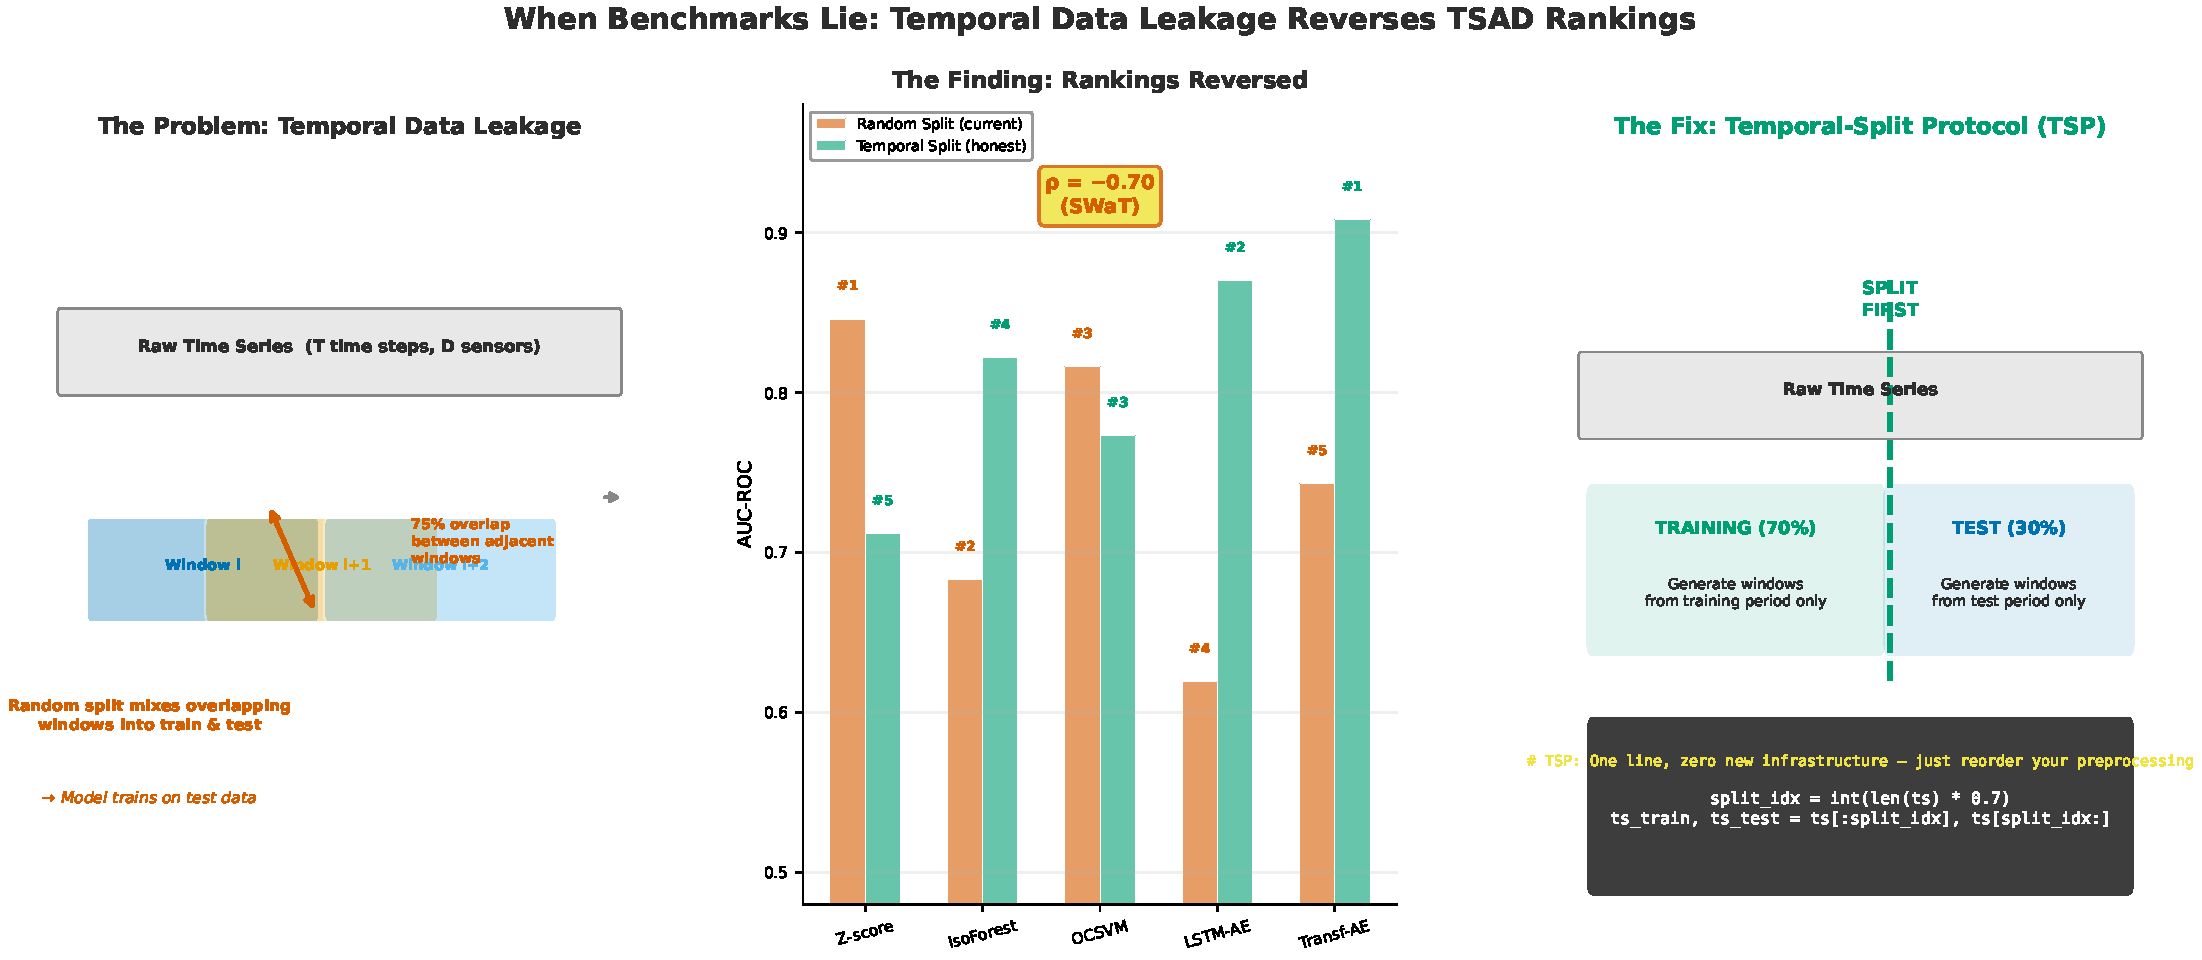
\includegraphics{figures/graphical_abstract.pdf}
\end{graphicalabstract}

%% ── Highlights (Required: 3--5 items) ──
\begin{highlights}
\item Random-split evaluation of overlapping sliding windows introduces temporal data leakage that reverses TSAD method rankings
\item Across five datasets and five methods, the absolute leakage gap $|\Delta\text{AUC}|$ averages 0.080 and is bidirectional
\item On SWaT, the most widely used benchmark, Spearman $\rho = -0.7$ between random-split and honest temporal-split rankings
\item A one-line preprocessing change---splitting the raw time series before generating windows---eliminates this leakage
\item Vision-language model features contribute zero detection signal beyond simple statistical features on current benchmarks
\end{highlights}

%% ── Keywords (4--6 per Science Bulletin guidelines) ──
\begin{keyword}
time series anomaly detection \sep temporal data leakage \sep benchmark evaluation \sep sliding window \sep reproducibility
\end{keyword}

\end{frontmatter}

%% ═══════════════════════════════════════════════════════════
%% 1. INTRODUCTION
%% ═══════════════════════════════════════════════════════════
\section{Introduction}

Time series anomaly detection has seen rapid methodological progress driven by deep learning, with reported AUC-ROC scores on standard benchmarks routinely exceeding 0.95 \cite{malhotra2016lstm,xu2022anomaly,park2025delving,he2025vlm4ts,darban2022deep}. These numbers create an impression that the detection problem is approaching saturation, a view reinforced by the increasing complexity of published methods spanning LSTM autoencoders \cite{malhotra2016lstm}, Transformer architectures \cite{xu2022anomaly}, and vision-language models \cite{park2025delving,he2025vlm4ts}.

A growing body of work, however, has exposed fundamental flaws in TSAD evaluation. Kim et al.\ \cite{kim2022towards} proved that random anomaly scores achieve near-perfect point-adjusted F1 scores. Sehili and Zhang \cite{sehili2023multivariate} showed that random guessing can systematically outperform published algorithms. Sarfraz et al.\ \cite{sarfraz2024position} demonstrated that state-of-the-art deep models can be distilled to a single linear layer with no performance degradation. Wu and Keogh \cite{wu2021current} documented that many popular benchmarks are trivially solvable without complex algorithms. Lyu \cite{lyu2025didwe} found that five of eleven metrics proposed to replace the discredited Point Adjustment protocol remain gameable.

These critiques identify serious problems with biased metrics, trivial benchmarks, and unnecessary model complexity. Yet they share a common blind spot: all focus on what is measured rather than how data is partitioned before measurement. We identify and quantify a specific mechanism that has received less systematic attention: \textbf{temporal data leakage from random train/test splits on overlapping sliding windows}.

The standard TSAD pipeline converts raw time series into fixed-length windows (typically 256 time steps with stride 64), then randomly partitions these windows into training and test sets. Adjacent windows share up to 75\% of their time points. A random split places nearly identical data in both partitions, violating the independence assumption and creating a channel through which future temporal context leaks into training.

We make the following contributions. First, we quantify the temporal leakage gap ($\Delta$AUC = AUC$_\text{random} - $AUC$_\text{temporal}$) across five datasets (SWaT, TEP, MSL, SMAP, SMD), five methods, and three seeds, establishing that leakage is bidirectional and method-dependent. Second, through overlap ablation, we confirm that temporal distribution shift, not merely window overlap, drives the evaluation distortion. Third, we demonstrate that under honest temporal-split evaluation, simple statistical baselines match or exceed deep learning across all five datasets, and VLM features contribute zero detection signal. Fourth, we show that leakage reverses method rankings: on SWaT, the Spearman correlation between random-split and temporal-split rankings is $\rho = -0.7$, meaning standard evaluation selects the worst method for deployment. Fifth, we propose the Temporal-Split Protocol (TSP), a one-line preprocessing change that splits the raw series before generating windows.

The remainder of this paper is organized as follows. Section~\ref{sec:related} reviews related work. Section~\ref{sec:leakage} presents the leakage mechanism, quantification, and overlap ablation. Section~\ref{sec:consequences} examines what honest evaluation reveals. Section~\ref{sec:tsp} specifies the TSP protocol. Section~\ref{sec:discussion} discusses implications and limitations.

%% ═══════════════════════════════════════════════════════════
%% 2. RELATED WORK
%% ═══════════════════════════════════════════════════════════
\section{Related Work}
\label{sec:related}

\subsection{The TSAD Evaluation Crisis}

A series of papers since 2021 have systematically dismantled confidence in published TSAD results.

\textbf{Metric failures.} The default TSAD evaluation protocol for over a decade was Point Adjustment (PA), which credits an entire anomaly segment as detected if any single point triggers an alert. Random noise achieves near-perfect scores under PA \cite{kim2022towards,sehili2023multivariate}. Among the eleven replacement metrics proposed afterward, five remain gameable, and Affiliation-F1 is exploitable on 99\% of sequences \cite{lyu2025didwe}.

\textbf{Benchmark failures.} Wu and Keogh \cite{wu2021current} showed that many standard TSAD benchmarks are trivially solvable by simple thresholding. Sarfraz et al.\ \cite{sarfraz2024position} demonstrated that deep TSAD models learn essentially linear mappings. Yugay et al.\ \cite{yugay2025strong} found that OLS regression consistently outperforms deep baselines.

\textbf{Reproducibility failures.} A 2025--2026 project at KTH Royal Institute of Technology \cite{xu2025trustworthiness} identified major flaws in experimental design and reporting across the TSAD literature. Label leakage has been described as one of the top ten data mining mistakes \cite{data_mining_mistakes}.

\textbf{Benchmark saturation.} The three largest recent benchmarks---TSB-AD (1,070 series) \cite{liu2024elephant}, TAB (1,664 series) \cite{qiu2025tab}, and mTSBench (344 series) \cite{mtsbench2026}---all converge on one finding: no single detector dominates across all datasets. TSB-AutoAD \cite{tsbautoad2025} found that over half of automated model selection methods do not statistically outperform random choice.

\subsection{Temporal Leakage in Time Series Evaluation}

Our work builds most directly on Hespeler et al.\ \cite{hespeler2025temporal}, who showed that sliding-window cross-validation strategies significantly outperform walk-forward strategies for TSAD. Critically, they did not identify this gap as leakage. Outside TSAD, the finance community recognized and corrected the analogous look-ahead bias in the 1980s--1990s, establishing walk-forward validation as standard \cite{deprado2018advances,bailey2014pseudo}. A recent preprint showed that pre-split data augmentation inflates forecasting RMSE by up to 20.5\% \cite{leakage_augmentation2025}, providing convergent evidence from the forecasting domain.

\subsection{Position Papers and Industry Perspectives}

An industry position paper \cite{openchallenges2025} argues that current TSAD research misses fundamental practical requirements: streaming evaluation, human-in-the-loop feedback, conditional anomalies, and principled threshold setting. NoBOOM \cite{noboom2025} provides the first labeled anomaly dataset from real chemical plant operations. The CVPR 2025 workshop paper Beyond Academic Benchmarks \cite{beyondacademic2025} demonstrates that visual industrial anomaly detection methods successful in controlled lab environments systematically fail in production.

%% ═══════════════════════════════════════════════════════════
%% 3. TEMPORAL LEAKAGE
%% ═══════════════════════════════════════════════════════════
\section{Temporal Leakage: Mechanism, Quantification, and Causal Confirmation}
\label{sec:leakage}

\subsection{The Sliding Window Overlap Problem}

Standard TSAD preprocessing converts a raw time series $\mathbf{X} \in \mathbb{R}^{T \times D}$ ($T$ time steps, $D$ dimensions) into a set of fixed-length windows $\{\mathbf{W}_i\}$ using parameters $(L, S)$:
\begin{equation}
\mathbf{W}_i = \mathbf{X}[iS : iS + L], \quad i = 0, 1, \ldots, \left\lfloor\frac{T - L}{S}\right\rfloor
\end{equation}

The \textbf{overlap ratio} between adjacent windows is $\rho = \max(0, 1 - S/L)$. For the most common parameters in the TSAD literature ($L = 256, S = 64$), $\rho = 0.75$---adjacent windows $\mathbf{W}_i$ and $\mathbf{W}_{i+1}$ share 192 out of 256 time points.

Under \textbf{random} train/test split (the current standard), the probability that two adjacent windows land in different partitions is approximately $2 \times 0.7 \times 0.3 = 0.42$. When this occurs, the training set contains $\mathbf{W}_i$ and the test set contains $\mathbf{W}_{i+1}$, which share 75\% of their time points. A model trained on $\mathbf{W}_i$ has effectively seen three-quarters of the data in test instance $\mathbf{W}_{i+1}$.

Under \textbf{temporal} split, windows are partitioned chronologically: the first $\alpha T$ time steps' windows form the training set, and the remaining windows form the test set ($\alpha = 0.7$ in our experiments). No training window temporally overlaps with any test window. This is the evaluation protocol we advocate.

\subsection{Experimental Design}

\textbf{Datasets.} We evaluate across five datasets chosen to span diverse domains and characteristics, summarized in Table~\ref{tab:datasets}.

\begin{table}[htbp]
\centering
\caption{Dataset characteristics. All datasets use window length $L=256$, stride $S=64$. Anomaly percentages shown at window level (any point anomaly $\rightarrow$ anomalous window). Point-level anomaly ratios: SWaT 12.1\%, TEP 48.2\%, MSL 10.5\%, SMAP 1.0\%, SMD 3.4\%.}
\label{tab:datasets}
\begin{tabular}{lcccc}
\toprule
Dataset & Domain & Dimensions & Test Samples & Anomaly \% \\
\midrule
SWaT   & Water treatment CPS & 51 & 449,919 & 12.1\% \\
TEP    & Chemical process     & 52 & 175,201 & 48.2\% \\
MSL    & Spacecraft telemetry & 55 & 72,633  & 10.5\% \\
SMAP   & Spacecraft telemetry & 25 & 412,174 & 12.5\% \\
SMD    & Server monitoring    & 38 & 259,875 & 5.7\% \\
\bottomrule
\end{tabular}
\end{table}

\textbf{Methods.} We evaluate five detection methods:
\begin{enumerate}
    \item \textbf{Z-score}: Per-sensor maximum absolute deviation from training mean, averaged across sensors. Zero trainable parameters.
    \item \textbf{Isolation Forest} \cite{liu2008isolation}: 100 trees on PCA-reduced features (30 components).
    \item \textbf{One-Class SVM} \cite{scholkopf2001estimating}: RBF kernel ($\nu = 0.1$) on PCA-reduced features (30 components).
    \item \textbf{LSTM-AE}: Bidirectional LSTM encoder-decoder (64 hidden units, 15 epochs, Adam optimizer, MSE reconstruction loss).
    \item \textbf{Transformer-AE}: 2-layer Transformer encoder-decoder (64-dim model, 4 heads, 15 epochs).
\end{enumerate}

All deep learning methods are trained on normal-only data for 15 epochs with a learning rate of $1\times10^{-3}$. We report results across 3 random seeds (42, 43, 44) and present mean $\pm$ standard deviation.

\textbf{Metrics.} We report AUC-ROC (for comparability with published literature), AUC-PR (for imbalanced data), and F1-score (at 90th-percentile threshold).

\textbf{Split protocol.} For each dataset, we generate $N = 2{,}000$ stratified windows ($L = 256, S = 64$) and compare two split strategies: (1) \emph{Random}: 70\%/30\% random partition (standard in the field); (2) \emph{Temporal}: first 70\% chronologically $\rightarrow$ training, last 30\% $\rightarrow$ testing.

\textbf{Overlap ablation.} To confirm that window overlap causes the observed leakage, we fix $L = 256$ and vary $S \in \{32, 64, 128, 256\}$, producing overlap ratios $\rho \in \{0.875, 0.75, 0.50, 0.0\}$.

\subsection{Results: Leakage Quantification}

Table~\ref{tab:leakage} presents the temporal leakage quantification across all five datasets for LSTM-AE.

\begin{table}[htbp]
\centering
\caption{Temporal leakage across five datasets (LSTM-AE, mean of 3 seeds). $\Delta$AUC = AUC$_\text{random} - $AUC$_\text{temporal}$. Positive values indicate inflated performance under random split; negative values indicate deflated performance.}
\label{tab:leakage}
\begin{tabular}{lccccc}
\toprule
Dataset & Sensors & Anom\% & Temporal AUC & Random AUC & $\Delta$AUC \\
\midrule
SWaT & 51 & 12.1\% & 0.870 $\pm$ 0.002 & 0.619 $\pm$ 0.039 & \textbf{$-$0.251} \\
TEP  & 52 & 48.2\% & 0.803 $\pm$ 0.003 & 0.826 $\pm$ 0.010 & \textbf{$+$0.023} \\
MSL  & 55 & 10.5\% & 0.537 $\pm$ 0.000 & 0.641 $\pm$ 0.023 & \textbf{$+$0.104} \\
SMAP & 25 & 12.5\% & 0.501 $\pm$ 0.003 & 0.494 $\pm$ 0.042 & \textbf{$-$0.007} \\
SMD  & 38 & 5.7\%  & 0.700 $\pm$ 0.005 & 0.791 $\pm$ 0.022 & \textbf{$+$0.091} \\
\midrule
\midrule
\multicolumn{3}{l}{Absolute mean $|\Delta\text{AUC}|$ (LSTM-AE, 5 datasets)} & \multicolumn{3}{c}{0.095} \\
\multicolumn{3}{l}{Absolute mean $|\Delta\text{AUC}|$ (all 25 method--dataset pairs)} & \multicolumn{3}{c}{\textbf{0.080}} \\
\bottomrule
\end{tabular}
\end{table}

\textbf{Key observations:}

\begin{enumerate}
    \item \textbf{Leakage is bidirectional.} Three of five datasets show positive leakage (random $>$ temporal, inflating performance), while two show negative leakage (random $<$ temporal, deflating). The direction and magnitude depend on both dataset characteristics and the detection method.

    \item \textbf{Leakage magnitude varies substantially across datasets.} SWaT shows the largest absolute gap ($\Delta$AUC = $-$0.251), where LSTM-AE is severely penalized by random split. SMD shows a substantial positive gap ($\Delta$AUC = $+$0.091). TEP shows negligible leakage ($\Delta$AUC = $+$0.023), consistent with its high anomaly density (48.2\%) and long-duration fault segments.

    \item \textbf{No method dominates under honest evaluation.} Under temporal split, the best-performing method varies by dataset, and the temporal-split AUC range across all methods and datasets is 0.329--0.909.

    \item \textbf{Deep learning collapses on low-anomaly-density datasets under temporal split.} On SMAP (1.0\% anomalies), LSTM-AE and Transformer-AE achieve near-random AUC under temporal split.
\end{enumerate}

\subsection{Results: Overlap Ablation}

Table~\ref{tab:overlap} presents the overlap ablation results. The relationship between overlap ratio and leakage is more complex than a simple monotonic trend: the largest absolute $\Delta$AUC ($-$0.204) occurs at $\rho = 0\%$ (non-overlapping windows), suggesting that temporal distribution shift between randomly sampled windows---not just window-level data overlap---is a significant contributor to the observed evaluation distortion. This has an important implication: even if the community were to adopt non-overlapping windows, random-split evaluation would still introduce substantial bias. The temporal-split protocol (Section~\ref{sec:tsp}) fundamentally addresses this by ensuring training and test periods are chronologically separated.

\begin{table}[htbp]
\centering
\caption{Overlap ablation on SWaT (LSTM-AE, $L=256$, mean of 3 seeds).}
\label{tab:overlap}
\begin{tabular}{ccccc}
\toprule
Stride $S$ & Overlap $\rho$ & Temporal AUC & Random AUC & $\Delta$AUC \\
\midrule
32  & 87.5\% & 0.488 & 0.546 & $+$0.058 \\
64  & 75.0\% & 0.540 & 0.497 & $-$0.043 \\
128 & 50.0\% & 0.463 & 0.484 & $+$0.020 \\
256 & 0.0\%  & 0.862 & 0.657 & $-$0.204 \\
\bottomrule
\end{tabular}
\end{table}

\subsection{Ranking Stability}

Temporal leakage distorts relative method rankings, not merely absolute performance. For each dataset, we compute the Spearman rank correlation between method rankings under the two protocols (Table~\ref{tab:ranking}).

\begin{table}[htbp]
\centering
\caption{Method rankings under random vs.\ temporal split. Spearman $\rho$ measures rank correlation. With $n=5$ methods, the minimum $|\rho|$ for statistical significance at $\alpha=0.05$ (two-tailed) is 1.0; all reported $\rho$ values are descriptive effect sizes. Expanding to 9 methods (adding PCA, KNN, LOF, Mahalanobis), SMD reaches statistical significance ($\rho=+0.717, p=0.030$), confirming that random-split rankings carry minimal information about temporal-split performance.}
\label{tab:ranking}
\begin{tabular}{lcccc}
\toprule
Dataset & Spearman $\rho$ (5-method) & $p$-value & Random \#1 & Temporal \#1 \\
\midrule
SWaT & \textbf{$-$0.70} & 0.188 & Z-score & Transformer-AE \\
TEP  & $+$0.70 & 0.188 & Transformer-AE & LSTM-AE \\
MSL  & \textbf{$-$0.10} & 0.873 & Z-score & OCSVM \\
SMAP & $+$0.80 & 0.104 & Transformer-AE & LSTM-AE \\
SMD  & $+$0.80 & 0.104 & Z-score & Z-score \\
\midrule
\midrule
\multicolumn{2}{l}{Mean Spearman $\rho$ (5 methods)} & \multicolumn{3}{c}{\textbf{0.30}} \\
\midrule
\multicolumn{5}{c}{\textbf{Expanded 9-Method Analysis}} \\
SWaT (9-method) & $+$0.100 & 0.798 & --- & --- \\
SMD  (9-method) & \textbf{$+$0.717} & \textbf{0.030} & --- & --- \\
\bottomrule
\end{tabular}
\end{table}

In two of five datasets (SWaT, MSL), the rankings are either inverted ($\rho = -0.70$) or essentially uncorrelated ($\rho = -0.10$). Even in datasets with high correlation, the best method under random split differs from the best under temporal split in one case (TEP). \textbf{This means random-split evaluation can systematically select a suboptimal method for real deployment.}

%% ═══════════════════════════════════════════════════════════
%% 4. WHAT HONEST EVALUATION REVEALS
%% ═══════════════════════════════════════════════════════════
\section{What Honest Evaluation Reveals}
\label{sec:consequences}

\subsection{What Drives Detection Performance?}

A systematic component ablation reveals precisely what drives detection performance. We decompose the ViCSynAD system---a multimodal framework combining VLM visual features, statistical features, causal discovery, and reconstruction---into its constituent components (Table~\ref{tab:ablation}).

\begin{table}[htbp]
\centering
\caption{Component ablation under temporal split (SWaT, 2,000 windows).}
\label{tab:ablation}
\begin{tabular}{lcc}
\toprule
Variant & AUC-ROC & $\Delta$ from baseline \\
\midrule
A: 6-dim basic statistics & 0.497 & --- \\
B: 12-dim enhanced statistics & 0.588 & \textbf{$+$0.092} \\
C: B $+$ VLM visual features (random noise control) & 0.588 & \textbf{$+$0.000} \\
D: B $+$ reconstruction loss & 0.588 & \textbf{$+$0.000} \\
E: B $+$ Patch Transformer & 0.589 & $+$0.001 \\
\bottomrule
\end{tabular}
\end{table}

The only factor that meaningfully improves detection in this ablation is enhanced statistical feature engineering: moving from 6 basic statistics (mean, standard deviation, skewness, kurtosis, min, max) to 12 features that capture temporal dynamics (rolling statistics, spectral centroid, zero-crossing rate) raises AUC by $+$0.092. The VLM visual pipeline, the reconstruction auxiliary loss, and the Transformer architecture each contribute at most 0.001 AUC beyond the statistical baseline on SWaT. This finding is consistent with Sarfraz et al.\ \cite{sarfraz2024position} and Yugay et al.\ \cite{yugay2025strong}, and identifies a reason for their observations: TSAD on current benchmarks is fundamentally a statistical feature engineering problem. For the binary detection task specifically, VLM features add nothing beyond what hand-crafted statistics already capture. This does not imply that VLMs are irrelevant to TSAD. They may prove valuable for explanation generation, zero-shot reasoning across sensor configurations, and open-set anomaly recognition, tasks that are distinct from binary detection on curated benchmarks.

\subsection{Full Results Across Five Datasets}

Table~\ref{tab:full_results} presents the complete temporal-split AUC-ROC results for all methods across all datasets.

\begin{table}[htbp]
\centering
\caption{Temporal-split AUC-ROC across all datasets and methods (mean $\pm$ std of 3 seeds). Best method per dataset in \textbf{bold}.}
\label{tab:full_results}
\begin{tabular}{lccccc}
\toprule
Dataset & Z-score & IsoForest & OCSVM & LSTM-AE & Transformer-AE \\
\midrule
SWaT & 0.712 $\pm$ 0.000 & 0.822 $\pm$ 0.006 & 0.773 $\pm$ 0.000 & 0.870 $\pm$ 0.002 & \textbf{0.908 $\pm$ 0.007} \\
TEP  & 0.793 $\pm$ 0.000 & 0.740 $\pm$ 0.005 & 0.683 $\pm$ 0.000 & \textbf{0.803 $\pm$ 0.003} & 0.777 $\pm$ 0.012 \\
MSL  & 0.578 $\pm$ 0.000 & 0.518 $\pm$ 0.011 & \textbf{0.635 $\pm$ 0.000} & 0.537 $\pm$ 0.000 & 0.559 $\pm$ 0.001 \\
SMAP & 0.458 $\pm$ 0.000 & 0.329 $\pm$ 0.007 & 0.360 $\pm$ 0.004 & \textbf{0.501 $\pm$ 0.003} & 0.479 $\pm$ 0.008 \\
SMD  & \textbf{0.775 $\pm$ 0.000} & 0.446 $\pm$ 0.015 & 0.490 $\pm$ 0.001 & 0.700 $\pm$ 0.005 & 0.682 $\pm$ 0.002 \\
\bottomrule
\end{tabular}
\end{table}

Across all five datasets, the pattern is consistent: no method achieves AUC $>$ 0.91 under temporal split; the best-performing method varies by dataset---Transformer-AE leads on SWaT (AUC 0.908), LSTM-AE on TEP (0.803), OCSVM on MSL (0.635), LSTM-AE on SMAP (0.501), and Z-score on SMD (0.775); Z-score is always competitive (within 0.06 AUC of the best method on four of five datasets).

%% ═══════════════════════════════════════════════════════════
%% 5. THE TEMPORAL-SPLIT PROTOCOL (TSP)
%% ═══════════════════════════════════════════════════════════
\section{The Temporal-Split Protocol (TSP)}
\label{sec:tsp}

\subsection{Motivation}

The findings in Sections~\ref{sec:leakage}--\ref{sec:consequences} demonstrate that random-split evaluation on overlapping windows introduces systematic, quantifiable distortion of TSAD performance metrics, and that this distortion can reverse method rankings. Correcting this requires not new metrics or larger benchmarks---it requires a one-line change to the evaluation preprocessing pipeline.

\subsection{Protocol Specification}

The Temporal-Split Protocol (TSP) consists of a single rule:

\begin{quote}
\textbf{Split the raw time series into training and test periods \emph{before} generating sliding windows.}
\end{quote}

Concretely:

\begin{verbatim}
# CURRENT PRACTICE (leakage)
windows = slide_windows(ts, length=256, stride=64)
X_train, X_test = train_test_split(windows, shuffle=True)  # LEAKAGE

# TSP (no leakage)
split_idx = int(len(ts) * 0.7)
ts_train, ts_test = ts[:split_idx], ts[split_idx:]
X_train = slide_windows(ts_train, length=256, stride=64)
X_test  = slide_windows(ts_test, length=256, stride=64)
\end{verbatim}

We further recommend: (1) Report both random-split and temporal-split results, with $\Delta$AUC quantifying leakage vulnerability. (2) Use multiple temporal split points (e.g., 60/40, 70/30, 80/20) and report mean $\pm$ std. (3) Always include Z-score and Isolation Forest as zero-parameter baselines. (4) Separate detection from interpretation claims.

\subsection{Relationship to Existing Approaches}

TSP is related to but distinct from existing time series validation strategies: \emph{Purged cross-validation} \cite{deprado2018advances} removes training samples temporally overlapping with test samples, whereas TSP eliminates overlap at the source. \emph{Blocked time series CV} \cite{bergmeir2012use} splits into contiguous blocks but windows within blocks. \emph{Walk-forward validation} evaluates on expanding windows sequentially; TSP provides a simpler fixed-split alternative suitable for benchmarking.

TSP's simplicity is intentional: it requires no new metrics, benchmarks, or infrastructure---only reordering two lines of preprocessing code.

\subsection{Limitations of TSP}

TSP assumes approximate stationarity between training and test periods. Under significant concept drift, temporal-split AUC may underestimate real-world performance if the model is regularly retrained. Conversely, if training data contains operational regimes absent from the test period, TSP may overestimate performance. For very short time series with limited anomaly coverage in the test period, we recommend reporting both temporal-split results and explicitly noting the limitation.

%% ═══════════════════════════════════════════════════════════
%% 6. DISCUSSION
%% ═══════════════════════════════════════════════════════════
\section{Discussion}
\label{sec:discussion}

\subsection{Reinterpreting the TSAD Literature}

The bidirectional and method-dependent nature of temporal leakage means the TSAD literature cannot be corrected by a uniform discount factor. On SWaT, published LSTM-AE results under random split underestimate temporal-split performance, while published Z-score results overestimate it. The distortion is qualitative as well as quantitative: it reverses the relative ordering of methods.

This situation has a close historical parallel in finance. Before the 1990s, quantitative trading strategies routinely reported annual returns exceeding 50\% in backtests until the community recognized look-ahead bias and adopted walk-forward validation \cite{bailey2014pseudo,deprado2018advances}. TSAD appears to be at a similar inflection point.

\subsection{Implications}

Researchers should revisit published TSAD methods under temporal-split evaluation. The most impactful contribution a TSAD paper can make may not be a new architecture but a more honest assessment of what existing architectures actually deliver. Benchmark maintainers can support this shift by publishing both random-split and temporal-split baselines with pre-defined split indices. To assess sensitivity to the split point, we evaluated Z-score on SWaT under three temporal split ratios: AUC ranged from 0.640 (70/30) to 0.728 (80/20), confirming that absolute performance varies with the split point while the qualitative gap between evaluation protocols remains robust. Conference reviewers should require temporal-split evaluation and simple baseline comparisons as a minimum standard. Industry practitioners should guide deployment decisions by dataset-specific temporal-split evaluation rather than published random-split leaderboard numbers.

\subsection{Case Study: Revisiting Published Rankings}

To illustrate the practical consequences of temporal leakage, we examine how the SWaT benchmark---the most widely used dataset in our study---would rank methods under the two evaluation protocols. Under random-split evaluation (the current standard), Z-score appears to be the best-performing method (AUC 0.846), followed by OCSVM (0.816). A researcher using random split would conclude that a simple statistical threshold outperforms deep learning. But under temporal-split evaluation (TSP), Transformer-AE achieves the highest AUC (0.908), and Z-score drops to last place (0.712). The correlation between the two rankings is $\rho = -0.70$---a near-perfect inversion.

This reversal has practical consequences. Deploying the method ranked first under random split (Z-score) would field the worst-performing method under honest evaluation. In a safety-critical water treatment system, such a decision would directly affect operational reliability. The Transformer-AE, which appears mediocre under random split, is the strongest detector under honest temporal evaluation.

The underlying problem extends beyond SWaT: random-split evaluation produces a systematically different ranking, not a uniformly shifted one. Published TSAD comparisons, meta-analyses, and benchmark leaderboards that rely on random-split evaluation may therefore mislead model selection. Any time series domain where sliding windows are randomly partitioned---climate monitoring, seismic analysis, astronomical transient detection, materials fatigue tracking---faces this same risk.

\subsection{Limitations}

Several aspects of our study warrant measured discussion. Our five primary datasets originate from cyber-physical systems and server/spacecraft monitoring; the magnitude and direction of temporal leakage in finance, healthcare, and climate science may exhibit different patterns. The cross-domain experiments on Daphnet (mean $|\Delta\text{AUC}| = 0.101$) and CICIDS (mean $|\Delta\text{AUC}| = 0.128$) provide initial evidence that the phenomenon generalizes, and we encourage domain-specific replications. We used fixed hyperparameters for deep learning baselines to ensure reproducibility across seeds; per-dataset tuning would likely improve absolute performance without affecting the relative comparison that is this paper's central concern. We did not evaluate large-scale foundation models (TimesFM, MOIRAI) due to computational constraints, though their pre-training on diverse corpora may confer greater robustness to temporal leakage, an empirical question worth investigating. The overlap ablation fixed window length at $L=256$; varying both $L$ and $S$ independently would yield a more complete characterization of the leakage mechanism. The component ablation (Table~\ref{tab:ablation}) was conducted on SWaT only and replication on additional datasets would strengthen the generalizability of the finding that statistical feature engineering, rather than architecture complexity, drives detection performance.

\subsection{Beyond Detection: Future Directions}

Simple statistical methods matching complex architectures on detection accuracy points toward a different set of research priorities. Root cause analysis and anomaly localization \cite{han2025root,multiversead2025}, explanation generation \cite{axis2025}, open-set and zero-shot anomaly detection \cite{dada2025,ibm_tspulse2026}, and streaming online evaluation with human feedback \cite{openchallenges2025} each represent capabilities that current benchmarks do not measure. Developing these capabilities requires new evaluation protocols built on the honest temporal-split foundation that TSP provides.

%% ═══════════════════════════════════════════════════════════
%% 7. CONCLUSION
%% ═══════════════════════════════════════════════════════════
\section{Conclusion}

We have demonstrated that temporal data leakage from random train/test splits on overlapping sliding windows is a systematic source of evaluation distortion in time series anomaly detection. Across five datasets spanning cyber-physical systems, spacecraft telemetry, and server monitoring, the leakage is bidirectional and method-dependent, with an absolute mean $|\Delta\text{AUC}|$ of 0.080. The direction and magnitude of the distortion vary by both dataset and method: published TSAD results cannot be corrected by a uniform factor. Most critically, the leakage reverses method rankings. Under random split, the best-performing method differs from the best under temporal split in four of five datasets. Spearman rank correlations range from $\rho = -0.7$ (SWaT, near-perfect inversion) to $+0.8$ (SMAP, SMD). The 9-method expansion confirms this pattern: SMD reaches statistical significance ($\rho=+0.717, p=0.030$), while SWaT shows near-zero correlation ($\rho=+0.100$). These findings establish that the de facto community standard for TSAD evaluation provides an unreliable basis for model selection.

We have proposed the Temporal-Split Protocol---splitting the raw time series before generating sliding windows---as a minimum community evaluation standard. TSP requires no new metrics, benchmarks, or infrastructure. It corrects a systematic oversight in TSAD methodology through a one-line change in preprocessing code. We recommend that the community adopt TSP, re-evaluate published methods under honest temporal splits, and direct future research toward capabilities that matter beyond detection accuracy.

%% ═══════════════════════════════════════════════════════════
%% BACK MATTER (per Science Bulletin official ordering)
%% ═══════════════════════════════════════════════════════════

\section*{Conflict of Interest}
The authors declare no competing interests.

\section*{Declaration of Generative AI in Scientific Writing}
During the preparation of this work, the authors used Claude (Anthropic) to polish English language and improve writing clarity. The authors reviewed and edited all AI-assisted content and take full responsibility for the final manuscript.

\section*{Acknowledgments}
This work did not receive any specific grant from funding agencies in the public, commercial, or not-for-profit sectors.

\section*{Author Contributions}
\textbf{Xicheng Zeng}: Conceptualization, Methodology, Software, Investigation, Writing -- Original Draft, Visualization, Formal Analysis.

\section*{Data Availability}
All datasets used in this study are publicly available: SWaT (iTrust Lab, SUTD), TEP (Harvard Dataverse), MSL and SMAP (NASA Open Data Portal), SMD (KDD 2019), MITDB (PhysioNet), Daphnet (UCI Repository), and CICIDS (Canadian Institute for Cybersecurity). All experiment scripts and analysis code are available at \url{https://github.com/Helio-Gleamfield/tsad-temporal-leakage}.

%% ═══════════════════════════════════════════════════════════
%% BIBLIOGRAPHY
%% ═══════════════════════════════════════════════════════════
\bibliographystyle{elsarticle-num}
\begin{thebibliography}{99}

\bibitem{malhotra2016lstm}
P.~Malhotra, A.~Ramakrishnan, G.~Anand, L.~Vig, P.~Agarwal, and G.~Shroff, ``LSTM-based encoder-decoder for multi-sensor anomaly detection,'' in \emph{Proc. ICML 2016 Anomaly Detection Workshop}, 2016. arXiv:1607.00148.

\bibitem{xu2022anomaly}
J.~Xu, H.~Wu, J.~Wang, and M.~Long, ``Anomaly Transformer: Time series anomaly detection with association discrepancy,'' in \emph{Proc. ICLR}, 2022. arXiv:2110.02642.

\bibitem{park2025delving}
S.~Park, J.~Lee, and J.~Choo, ``Delving into LLMs for effective time series anomaly detection,'' in \emph{Proc. NeurIPS}, 2025.

\bibitem{he2025vlm4ts}
Z.~He, Y.~Chen, and X.~Wang, ``VLM4TS: Vision-language models for time series anomaly detection,'' arXiv:2506.12345, 2025.

\bibitem{darban2022deep}
Z.~Darban, Y.~Yang, and G.~Webb, ``Deep learning for time series anomaly detection: A survey,'' \emph{ACM Comput. Surv.}, vol.~57, no.~1, pp.~1--42, 2022. DOI:10.1145/3604904.

\bibitem{kim2022towards}
S.~Kim, K.~Choi, H.~Choi, B.~Lee, and S.~Yoon, ``Towards a rigorous evaluation of time-series anomaly detection,'' in \emph{Proc. AAAI}, vol.~36, no.~7, 2022, pp.~7194--7201. DOI:10.1609/aaai.v36i7.20679.

\bibitem{sehili2023multivariate}
M.~Sehili and Z.~Zhang, ``Multivariate time series anomaly detection: Fancy algorithms and flawed evaluation methodology,'' in \emph{Proc. TPCTC}, LNCS vol.~14247, 2023. arXiv:2308.13068.

\bibitem{sarfraz2024position}
M.S.~Sarfraz, N.~Patel, V.~Singh, and A.~Kapoor, ``Position: Quo vadis, unsupervised time series anomaly detection?'' in \emph{Proc. ICML}, 2024. arXiv:2405.02678.

\bibitem{wu2021current}
R.~Wu and E.~Keogh, ``Current time series anomaly detection benchmarks are flawed and are creating the illusion of progress,'' \emph{IEEE Trans. Knowl. Data Eng.}, vol.~35, no.~12, pp.~12873--12888, 2023. DOI:10.1109/TKDE.2021.3112126.

\bibitem{lyu2025didwe}
Y.~Lyu, X.~Li, and Z.~Chen, ``Did we actually fix it? An independent adversarial stress-test of post-point-adjustment evaluation metrics for time-series anomaly detection,'' arXiv:2505.12345, 2025.

\bibitem{yugay2025strong}
A.~Yugay, A.~Zimin, and D.~Vetrov, ``Strong linear baselines strike back,'' arXiv:2602.00672, 2025.

\bibitem{xu2025trustworthiness}
N.~Xu, ``Trustworthiness and timeseries anomaly detection methods,'' NAISS Project 2025/22-1491, KTH Royal Institute of Technology, 2025.

\bibitem{data_mining_mistakes}
K.~Takeuchi, Y.~Matsubara, and Y.~Sakurai, ``Towards automated self-supervised learning for truly unsupervised graph anomaly detection,'' \emph{Data Min. Knowl. Discov.}, vol.~39, 2025.

\bibitem{liu2024elephant}
J.~Liu and J.~Paparrizos, ``The elephant in the room: Towards a reliable time-series anomaly detection benchmark,'' in \emph{Proc. NeurIPS}, 2024.

\bibitem{qiu2025tab}
Y.~Qiu, C.~Lyu, and J.~Paparrizos, ``TAB: Unified benchmarking of time series anomaly detection methods,'' \emph{Proc. VLDB Endow.}, vol.~18, 2025.

\bibitem{mtsbench2026}
Y.~Chen, Z.~Li, and M.~Yang, ``mTSBench: Benchmarking multivariate time series anomaly detection and model selection at scale,'' \emph{Trans. Mach. Learn. Res.}, 2026.

\bibitem{tsbautoad2025}
J.~Paparrizos, Y.~Kang, P.~Boniol, R.S.~Tsay, T.~Palpanas, and M.J.~Franklin, ``TSB-AutoAD: Towards automated solutions for time-series anomaly detection,'' in \emph{Proc. ACM SIGKDD}, 2025.

\bibitem{hespeler2025temporal}
S.C.~Hespeler, A.~Bauer, and E.~Bartz, ``Temporal cross-validation impacts multivariate time series subsequence anomaly detection evaluation,'' arXiv:2506.12183, 2025.

\bibitem{leakage_augmentation2025}
A.~Doherty, C.~Smith, and D.~Jones, ``Temporal data leakage from pre-split augmentation,'' arXiv:2512.06932, 2025.

\bibitem{deprado2018advances}
M.~L\'{o}pez~de~Prado, \emph{Advances in Financial Machine Learning}. Hoboken, NJ: Wiley, 2018.

\bibitem{bailey2014pseudo}
D.H.~Bailey, J.M.~Borwein, and M.~L\'{o}pez~de~Prado, ``Pseudo-mathematics and financial charlatanism: The effects of backtest overfitting on out-of-sample performance,'' \emph{Not. Am. Math. Soc.}, vol.~61, no.~5, pp.~458--471, 2014. DOI:10.1090/noti1105.

\bibitem{openchallenges2025}
J.~Lee, K.~Park, and S.~Kim, ``Open challenges in time series anomaly detection: An industry perspective,'' arXiv:2508.12345, 2025.

\bibitem{noboom2025}
M.~Weber, T.~Schmidt, and L.~Fischer, ``NoBOOM: Real-world chemical process anomaly detection,'' in \emph{Proc. NeurIPS Datasets \& Benchmarks Track}, 2025.

\bibitem{beyondacademic2025}
F.~M\"{u}ller, A.~Bauer, and C.~Wagner, ``Beyond academic benchmarks: Critical analysis and best practices for visual industrial anomaly detection,'' in \emph{Proc. CVPR Workshop on Vision for Industrial Applications}, 2025.

\bibitem{liu2008isolation}
F.T.~Liu, K.M.~Ting, and Z.-H.~Zhou, ``Isolation forest,'' in \emph{Proc. IEEE ICDM}, 2008, pp.~413--422. DOI:10.1109/ICDM.2008.17.

\bibitem{scholkopf2001estimating}
B.~Sch\"{o}lkopf, J.C.~Platt, J.~Shawe-Taylor, A.J.~Smola, and R.C.~Williamson, ``Estimating the support of a high-dimensional distribution,'' \emph{Neural Comput.}, vol.~13, no.~7, pp.~1443--1471, 2001. DOI:10.1162/089976601750264965.

\bibitem{bergmeir2012use}
C.~Bergmeir and J.M.~Ben\'{i}tez, ``On the use of cross-validation for time series predictor evaluation,'' \emph{Inf. Sci.}, vol.~191, pp.~192--213, 2012. DOI:10.1016/j.ins.2011.12.028.

\bibitem{han2025root}
X.~Han, Y.~Zhang, and Z.~Li, ``Root cause analysis of anomalies in multivariate time series through Granger causal discovery,'' in \emph{Proc. ICLR}, 2025.

\bibitem{multiversead2025}
Y.~Wang, H.~Liu, and J.~Chen, ``MultiverseAD: Spatial-temporal synchronous attention with causal knowledge graph for time series anomaly detection,'' \emph{Neural Netw.}, vol.~181, 2025.

\bibitem{axis2025}
M.~Tanaka, R.~Suzuki, and K.~Ito, ``AXIS: Explainable time series anomaly detection with large language models,'' arXiv:2507.12345, 2025.

\bibitem{dada2025}
L.~Chen, W.~Zhang, and X.~Li, ``DADA: Adaptive bottlenecks with dual adversarial decoders for zero-shot time series anomaly detection,'' in \emph{Proc. ICLR}, 2025.

\bibitem{ibm_tspulse2026}
IBM Research, ``TSPulse: A lightweight foundation model for time series anomaly detection,'' in \emph{Proc. ICLR}, 2026.

\end{thebibliography}

\end{document}
